\chapter{Používateľské rozhranie}
\label{pouzivatelske_rozhranie}

Pre kontrolu funkčnosti nášho systému postačuje aj zmena zdrojových kódov.
Pre lepšiu použiteľnosť by však bolo vhodné vytvoriť nejaký druh prostredia pre používateľa.
Pre lepšiu prácu s naším systémom sme vytvorili grafické používateľské rozhranie.

Na začiatku nášho návrhu bola analýza už existujúcich programov, ktoré majú podobnú funkcionalitu.
Nakoľko systém, ktorý by generoval obrázky z hudobných skladieb neexistuje, ako predloha nám slúžila aplikácia Deep Dream Generátor, ktorá upravuje obrázky použitím algoritmov strojového učenia.

\section{Konceptuálny model}
Po analýze existujúcich riešení sme sa rozhodli, že naše grafické rozhranie bude poskytovať možnosť výberu skladby a následného výberu úseku skladby, z ktorého sa má generovať obrázok.
Na obrázku \ref{kon_model} je vidieť, že používateľ ("Človek") má prístup do galérie s obrázkami, ktoré môže mazať podľa svojho uváženia.
\begin{figure}[!ht]
	\centering 
	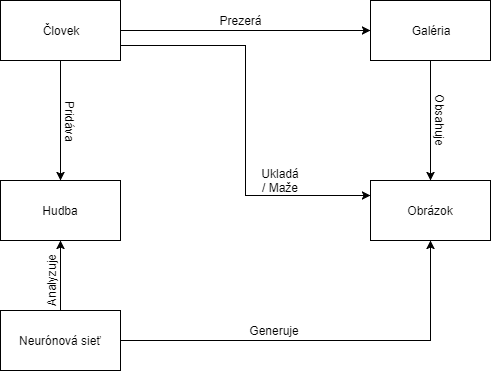
\includegraphics[height=.5\textwidth]{figures/km} 
	\caption{Konceptuálny model.} 
	\label{kon_model}
\end{figure}
Z tohto modelu je jasné, že generovanie obrázkov je priamočiare.
Človek vyberie hudbu, podľa ktorej sa má generovať, a náš systém, ktorý využíva neurónovú sieť, analyzuje skladbu a následne vygeneruje nový obrázok, ktorý sa uloží do galérie.

\section{Diagram postupnosti obrazoviek}

\begin{figure}[!ht] 
	\centering 
	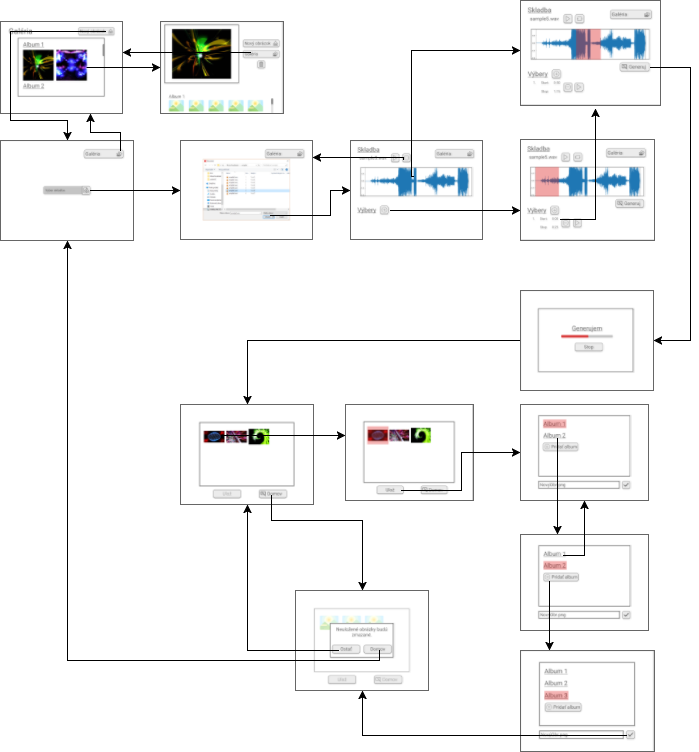
\includegraphics[height=.5\textwidth]{figures/ssq} 
	\caption{Diagram postupnosti obrazoviek.} 
	\label{ssq}
\end{figure}

Náš návrh je prehľadne vidno na diagrame postupnosti obrazoviek (Obr. \ref{ssq}).
Pri spustení sa otvorí stránka s galériou, z ktorej následne je možné prejsť na samotné generovanie nových obrázkov.
Proces vytvárania je rozdelený na tri sekcie, výber skladby, nastavenia úsekov skladby, podľa ktorých sa generovanie uskutočňuje, a samotné generovanie.
Po vytvorení nových obrázkov má používateľ možnosť uloženia do albumu.
V ponuke má zoznam už existujúcich albumov, no môže vytvoriť aj nový album.

\section{Iteratívny vývoj v prototypoch}
Návrh používateľského rozhrania sme vytvárali v dvoch cykloch.
Prototypy boli vytvorené pomocou nástroja Figma.
Každý prototyp bol otestovaný, a pre každý bolo vypočítané skóre použiteľnosti.

Oba prototypy testovali traja rôzny ľudia.
Vzorku účastníkov testu tvorili 20 až 25 roční študenti, ktorí nemali znalosti o tom ako má systém fungovať.
Priemerné skóre použiteľnosti pre prvý prototyp bolo 43,3 a pre druhý 55.

Po prvom testovaný nám bolo jasné, že používatelia nerozumeli nepopísaným tlačidlám a mali problém sa zorientovať na úvodnej ploche.
Po úpravách sa skóre rozhrania zlepšilo ale bolo stále jasné, že bežný používateľ nerozumie slovníku, ktorý sme použili a nevie čo má robiť.
Pri vytváraní finálneho funkčného prototypu sme sa snažili vyhnúť všetkým problémom a zlepšiť zrozumiteľnosť systému.


Vytvorenie prototypov a testovanie nám dalo lepšiu predstavu ako má finálny produkt vyzerať aby bol použiteľný.
Zároveň sme zistili, že chápanie systému, aj napriek jeho minimalistickému rozhraniu, je pre bežných používateľov prakticky neexistujúce.
Využitie metódy testovania použiteľnosti nám ale pomohlo rýchlo nájsť nedostatky v našom návrhu a zlepšiť celkovú kvalitu grafického používateľského rozhrania.
